\section{Capacitive prototypes from related work}
While I already have presented capacitive systems in the related work section, they are briefly revisited here, to classify them given the specified application domains. Similar to the created prototypes I will give some additional detail regarding their measuring layout and data processing. The prototypes are shortly listed in Table \ref{tab:related_cap_proto}. This additional information will be used to give a more informed discussion of benefits and limitations of capacitive proximity sensing technology in smart environments and will contribute to the set of guidelines for developers of capacitive sensing applications.

% Table generated by Excel2LaTeX from sheet 'Tabelle1'
\begin{table}[htbp]	
	\centering
  \footnotesize
  \caption{Measuring layout and data processing of different prototypes from related works}
    \begin{tabularx}{\linewidth}{Xp{3.5cm}Xp{3.5cm}p{3.5cm}}
    \toprule
    \textbf{Name} & \textbf{Description} & \textbf{Application Areas} & \textbf{Measuring Layout} & \textbf{Data Processing} \\
    \midrule
    \textbf{SensFloor \cite{lauterbach2009}} & System for indoor localization and fall detection as floor underlay & Indoor Localization & Loading mode, variable number of sensors based on area size & Individual coding of zones on floor - analysis of activity based on trajectories \\
    \textbf{TileTrack \cite{Valtonen2009a}} & Indoor localization using transmitters below floor and receiver electrodes in wall or furniture & Indoor Localization & Transmit mode, large transmitter electrodes below floor, different receiving electrodes & Location by calculating center-of-gravity on most active tiles \\
    \textbf{Touché \cite{Sato2012}} & Swept-frequency sensing to detect different types of touches on a conductive material & Smart Appliances & Swept-frequency sensing, single electrode & SVM classification using features in different frequency ranges \\
    \textbf{Botanicus Interactus \cite{poupyrev2012botanicus}} & Using plant tissue as conductive material as application for swept-frequency sensing & Smart Appliances & Swept-frequency sensing, electrode coupled to plant tissue & SVM classification of touches that are transferred to input events \\
    \textbf{HandSense \cite{wimmer2009handsense}} & Using capacitive sensors to detect grasp style & Smart Appliances & Four loading mode sensors on CapToolKit & Classification of holding styles based on threshold levels \\
    \textbf{Active capacitive sensing \cite{cheng2010active}} & Conductive textile electrodes to sense different parameters of the human body, based on location & Physiological Sensing & Loading mode, single electrode attached to body part & Different filtering methods, based on electrode position, activity classification using LDA \\
    \textbf{Spread spectrum sensor \cite{MacLachlan2004}} & Single electrodes using a spread spectrum technique for improved sensitivity & Physiological Sensing & Loading mode, single electrode placed remotely & Spread spectrum technique to improve SNR, amplitude measurement for respiratory rate \\
    \textbf{School of Fish \cite{smith1999thesis}} & Array of shunt mode sensors that can track 3D position and orientation of two hands  & Gesture Interaction & Shunt mode, flexible array of sensors & Modeling hands as collection of spheres and fit into area based on sensor values and position \\
    \textbf{Thracker \cite{Wimmer2006}} & Four electrodes placed around display that can sense spatial position of hand in front of display and certain gestures & Gesture Interaction & Loading mode, four electrodes placed spatially around display & Position based on distance to electrodes or gesture based on nearest object to electrode \\
    \textbf{Transparent electric field sensor \cite{le2014low}} & Transparent shunt mode array enabling near distance gesture interaction above mobile devices & Gesture Interaction & Shunt mode, four receiver electrodes & Positioning based on single proximity values and random decision forest learning \\
    \bottomrule
    \end{tabularx}%
  \label{tab:related_cap_proto}%
\end{table}%

\subsection{Indoor localization}
One example system based on capacitive sensing is the previously presented TileTrack that uses a combination of transmit mode and center-of-gravity calculation between different floor tiles to calculate the position of multiple persons \cite{Valtonen2009a}. They are using special floor tiles comprised of chipboard and a steel layer. The steel layer acts as transmitting electrode that is coupled to persons moving above it. The initial system used wire and plate electrodes that were integrated into a wall and running to a height of 1.90 m, thus ensuring receiving the field transmitted by tall persons. In order to properly localize a person the readings of multiple tiles relative to a single receiving electrode are combined. Similar to CapFloor (\ref{ch:prot_capfloor}) only passive materials are used below the floor level and the measurement systems can be hidden on the sides, however it requires large tile electrodes, thus it is mostly suited for hidden floor systems.

A second, already commercialized system is SensFloor that uses an integrated solution of capacitive sensors and wireless communication hidden below a floor covering that is able to detect the position of several users and other parameters such as falls, based on analyzing activity above single sensor areas or the movement trajectories over time \cite{lauterbach2009}. The sensors work in loading mode and track activity in specific areas that are bordered by a sensing wire circle. Eight areas are attached to a single sensor, comprising a rectangular tile. The system is designed as a floor underlay, with power supplies being attached on the side and the single sensors communicating wireless to a base station. While this setup allows a high resolution, it is fairly expensive to build and potentially difficult to maintain. 

\subsection{Smart Appliances}
Sato et al. have presented Touché, a swept-frequency capacitive sensor that allows distinguishing different types of touches on any suitable surface and medium \cite{Sato2012}. Some examples include recognizing different hand postures in liquids and touching different body parts to control mobile devices. Their system is based on analyzing a broader range of frequencies that have a different effect on the resulting capacitance. Using a classification method they are able to distinguish different categories of events. It supports an arbitrary number of electrode categories, yet only one single sensor attached to the measurement circuit. One additional feature is placing the electrode next to a conductive medium, such as water. Another example of this technology is touching different parts of a plant to control an interactive art installation  \cite{poupyrev2012botanicus}, showing the versatility of this sensing technology.

HandSense by Wimmer and Boring uses four loading mode electrodes placed around a box mimicking a mobile phone to detect different grasping styles. The electrodes are made of tin sheet and sized 30x15 mm and placed on both small sides of the plastic box. Using different thresholds for "No proximity", "Near", "On hand", "Gripped" and "Held" they are able to classify six different types of holding the phone with varying accuracy. The basic idea is to use the grasping style as additional input device, e.g. by switching thumb-based interface items, when it is held in different hands.

\subsection{Physiological sensing}
Capacitive proximity sensors can be used to measure various physiological parameters that are related to movement of different body parts, including internal organs, most notably the heart. Cheng et al. have presented a system that allows measuring motions and shape changes of body parts using capacitive sensors embedded in garment \cite{cheng2010active}. They combined four sensors based on loading mode that were exposed to electrodes made from conductive thread. They were attached to different body parts, including chest, wrist, upper legs and neck. According to position different forms of activities can be recognized, such as locomotion for the leg electrodes or swallowing for the neck electrodes. Additionally, the neck system could be used to detect the respiratory rate for some individuals. 

\begin{figure}[ht]
\centering
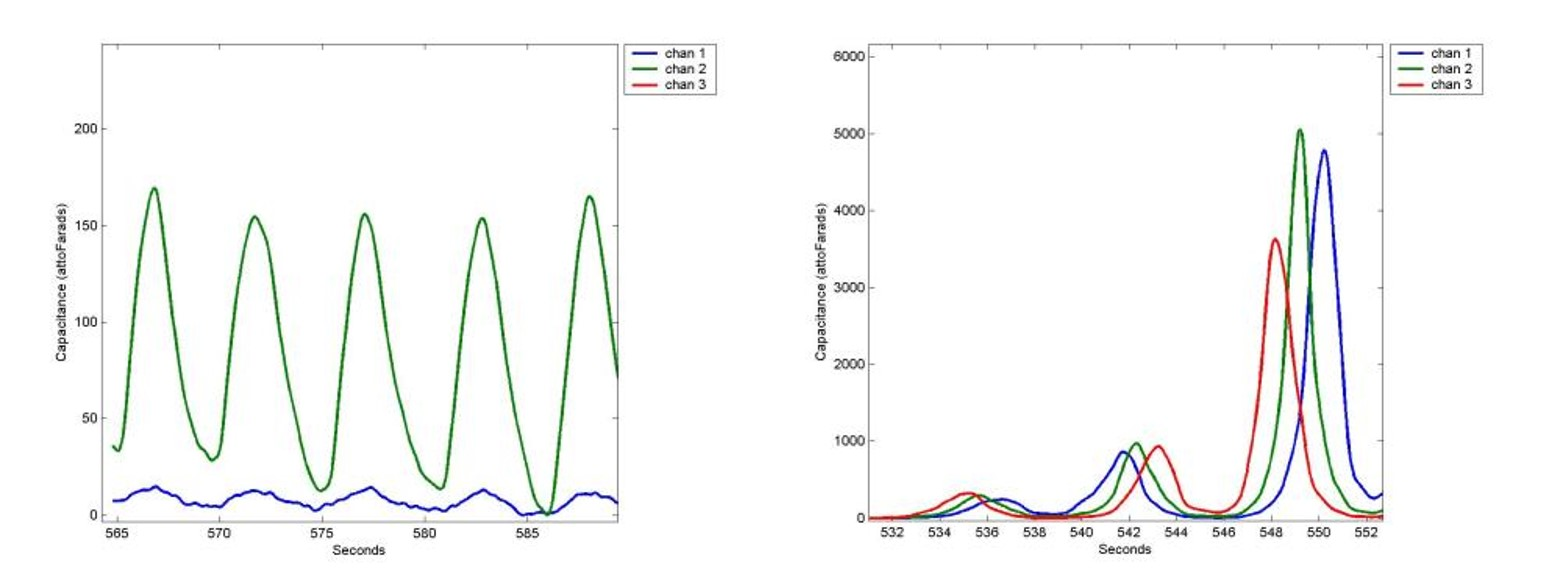
\includegraphics[width=0.8\textwidth]{images/spread_breath}
\caption{\emph{Left:}Spread spectrum capacitive sensor detecting respiration 30 cm (green) and 90 cm (blue) from chest. \emph{Right:} Same sensor detecting person walking by at 100 cm (left), 70 cm (middle) and 35 cm (right) \cite{MacLachlan2004}}
\label{fig:spread_breath}
\end{figure}

MacLachlan presented a system that detects the respiratory rate of a person lying on a bed from a distance of 30 cm using a single electrode and a highly sensitive sensing method based on spread spectrum methods that are commonly used in wireless communication \cite{MacLachlan2004}. Using a single electrode of 14x56 mm and the coding method he is able to detect very small capacitance changes. Figure \ref{fig:spread_breath} shows on the left the changes in capacitance caused by chest movement at a distance of 30 cm, respectively 90 cm from the moving chest. The response of three different sensors to a person passing at a distance of 100 cm, 70 cm and 35 cm can be seen in Figure \ref{fig:spread_breath} on the right. The system requires coding hardware next to the electrode, thus making it more complicated to manufacture, as opposed to the previous systems.

\subsection{Gestural interaction}
The School of Fish by Smith, is a shunt mode system that he developed in the scope of his PhD thesis and the basis for most of the capacitive sensor research at MIT in the 1990s \cite{smith1999thesis}. Comprised of a collection of hexagonal copper electrodes distinguished into senders and receivers. Larger arrays are able to detect position and orientation of two hands moving at a distance above it. Though it was not used for the school of fish the system could easily placed below non-conductive materials, e.g. integration into a table. The hands are modeled using a collection of spheres, enabling a calculation of the orientation.

Thracker by Wimmer et al. uses four electrodes placed around a display to detect the movement of a hand in proximity \cite{Wimmer2007a}. The electrodes are angled away from the screen to improve the resolution at a distance. Two different modes were evaluated. One tracked the position of the hand in front of the screen, while the second one investigated pick and drop gestures. 

A recent work by Le Goc et al. is based on the dedicated GestIC capacitive gesture tracking microchip \cite{le2014low}. Using transparent electrodes in shunt mode they are able to precisely track the 3D position of fingers moving in the electric field. The electrodes are based on an ITO layer on acrylic glass placed above a mobile phone. A second ITO layer is used to shield from interference generated by the capacitive touch screen of the phone. They use a random decision forest method to detect the position of a finger.


 
